\documentclass[]{IEEEtran}

\title{TLM description and integration on a Virtual Platform of a Single-Precision Floating-point IEEE 754 Multiplier}
\author{Fabio Chiarani - VR445566}

\usepackage{graphicx}
\usepackage[british]{babel}
\usepackage{multicol}

\usepackage{tikz}

\usepackage{pgf-umlsd}
\usetikzlibrary{arrows,automata, positioning}
\usepackage[latin1]{inputenc}


\usepackage{forest}
\usepackage{xcolor}
\usepackage{listings}
\usepackage{booktabs}
\usepackage{hyperref}
\usepackage{pgfplots}
\usepackage{rotating}

\begin{document}
	\maketitle
	
	\begin{abstract}
		The following document illustrates how an IEEE 754 single precision floating-point was simulated through different levels of abstraction with SystemC TLM: it was then simulated through the RTL, AT, LT and UT levels. The simulation consists of random multiplication tests repeated from $10^3$ to $10^9$ times, reporting and commenting on the data obtained. In a second phase the multiplier defined in Verilog and VHDL was connected to an existing virtual platform (COM6502-Splatters) verifying its functionality through the Vivado simulation.
	\end{abstract}
	
	\section{Introduction}
The following document illustrates how an IEEE 754 single precision floating-point was simulated through different levels of abstraction with SystemC TLM 2.0: it was then simulated through the different coding styles such as AT, LT and UT levels comparing it to the RTL (SystemC RTL description)  simulation. The simulation consists of multiplication tests repeated from $10^3$ to $10^9$ times, reporting and commenting data obtained. We want to see how the difference in abstraction improves and/or worsens the simulation time. In a second phase the multiplier defined in Verilog and VHDL on the previus report, was connected to an existing virtual platform (COM6502-Splatters) verifying its functionality through the Vivado simulation.

	The \hyperref[sec:Background]{'Background'} section gives some information about SystemC TLM and the Virtual Platfom pro and cons. 
	
	The Section \hyperref[sec:impl]{'TLM Implementation'} shows how the TLM descriptions is created for RTL, AT, LT and UT levels, reporting the data obtained from the simulations.
	
	The Section \hyperref[sec:vp]{'Virtual Platform Integration'} shows how the HDL multiplier is connected to the COM6502-Splat platform, reporting the data obtained from the platform simulation.

	\section{Background}
	\label{sec:Background}
	Platform-based design is the creation of (stable) microprocessor-based architectures, which can be quickly extended and modified for a set of applications, and given to consumers for rapid development. TLM is a golden model  which describes the design with the transactions (\textit{a transaction is the transfer of data from one module to another, represented by a generic payload, through primitive functions}) annotation and makes possible the verification and simulation on a layer above the RTL. 
	The TLM description is used for the device performance exploration, and running the software on a virtual platform (VP) of the hardware platform, it optimizes the software verification and makes a fast simulation available before the RTL implementation.
	
	SystemC-TLM \cite{SystemC-TLM} is a SystemC version that supports the TLM description. The use cases, which lead to choosing a TLM solution are the development of a faster software, an architectural performance analysis and hardware verification.
	SystemC-TLM provides different code-styles (which are standardized on SystemC-TLM 2.0):
	\begin{itemize}
		\item LT (Loosely-timed):  that has the details of how long it takes to boot up an OS and run a multicore system. It has a limited number of context-switch to 2: start and end of a transaction.
		\item AT (Approximately-timed): it is suitable for performance analysis and architectural exploration. The processes follow step by step with the simulation time and have 4 events: start and end of the request and, start and end of the response.
	\end{itemize}
	Another timing annotation is the UT (untimed) where time is not important.
	SystemC-TLM provides different interfaces based on the choice of the style of code adopted for allows the transaction between the initiator and a target:
	\begin{itemize}
		\item Blocking transport: used inside LT description, which has the time annotation on the socket; it uses only the forward path.
		\item Non-blocking transport: used inside AT description, which has the time and the transaction-phase on the socket; it can be used both on forward and backward path. The non-blocking transport is used when you want to specify more in details the interactions between the target and the initiatior.
	\end{itemize}


COM6502-Splatters is a virtual platform composed by: CPU MOS 6502 (1975) with 16 bit addressing (16KB ROM, 16KB RAM) and 8 bit data width; Memory with ROM in one single bank, RAM splitted in 8 different blocks to enable multi read/write operations and a Clock divider that manage MMIO operation between Peripherals, Memory and manage multiple write on same cell between CPU and MMIO Interface; and a BUS ARM APB (Advanced Peripheral Bus) that supports up to 8 peripherals; an IO Module used to request or send data out from the platform.
The use of platforms and/or virtual platforms allows to have a more general environment as well as only the hardware component. Another feature, thanks to the SystemC TLM 2.0 standard, let to reuse and/or use components already created to the platform reducing the time to market.

	\begin{center}


\tikzset{every picture/.style={line width=0.75pt}} %set default line width to 0.75pt        

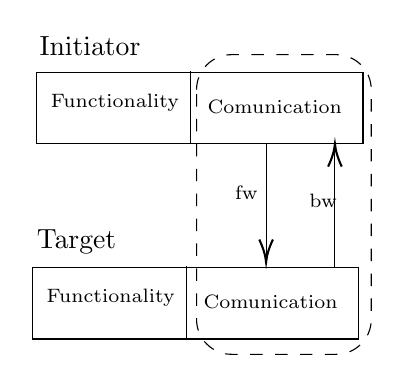
\begin{tikzpicture}[x=0.75pt,y=0.75pt,yscale=-1,xscale=1]
%uncomment if require: \path (0,213); %set diagram left start at 0, and has height of 213

%Shape: Rectangle [id:dp9211023518838333] 
\draw   (26.25,60.54) -- (183.5,60.54) -- (183.5,95) -- (26.25,95) -- cycle ;
%Straight Lines [id:da964059389744333] 
\draw    (100.5,60) -- (100.5,95) ;


%Rounded Rect [id:dp32759511217881776] 
\draw  [dash pattern={on 4.5pt off 4.5pt}] (103.33,68.83) .. controls (103.33,59.54) and (110.87,52) .. (120.17,52) -- (170.67,52) .. controls (179.96,52) and (187.5,59.54) .. (187.5,68.83) -- (187.5,179.54) .. controls (187.5,188.84) and (179.96,196.37) .. (170.67,196.37) -- (120.17,196.37) .. controls (110.87,196.37) and (103.33,188.84) .. (103.33,179.54) -- cycle ;
%Straight Lines [id:da5903625580084783] 
\draw    (136.83,95) -- (136.83,150) ;
\draw [shift={(136.83,152)}, rotate = 270] [color={rgb, 255:red, 0; green, 0; blue, 0 }  ][line width=0.75]    (10.93,-3.29) .. controls (6.95,-1.4) and (3.31,-0.3) .. (0,0) .. controls (3.31,0.3) and (6.95,1.4) .. (10.93,3.29)   ;

%Straight Lines [id:da970665910373827] 
\draw    (170,97) -- (170,154.67) ;

\draw [shift={(170,95)}, rotate = 90] [color={rgb, 255:red, 0; green, 0; blue, 0 }  ][line width=0.75]    (10.93,-3.29) .. controls (6.95,-1.4) and (3.31,-0.3) .. (0,0) .. controls (3.31,0.3) and (6.95,1.4) .. (10.93,3.29)   ;
%Shape: Rectangle [id:dp7542715476279406] 
\draw   (24.25,154.54) -- (181.5,154.54) -- (181.5,189) -- (24.25,189) -- cycle ;
%Straight Lines [id:da27707363231574844] 
\draw    (98.5,154) -- (98.5,189) ;



% Text Node
\draw (52,48) node   [align=left] {Initiator};
% Text Node
\draw (64,75) node   [align=left] {{\scriptsize Functionality}};
% Text Node
\draw (141,77) node   [align=left] {{\scriptsize Comunication}};
% Text Node
\draw (45.5,142) node   [align=left] {Target};
% Text Node
\draw (127.33,118.33) node  [font=\scriptsize] [align=left] {fw};
% Text Node
\draw (164.33,122.33) node  [font=\scriptsize] [align=left] {bw};
% Text Node
\draw (62,169) node   [align=left] {{\scriptsize Functionality}};
% Text Node
\draw (139,171) node   [align=left] {{\scriptsize Comunication}};


\end{tikzpicture}


	
	\end{center}

	
	\section{TLM Implementation}
	\label{sec:impl}
		After analyzing the required specifications, it has been chosen to implement first the TLM description of the IEEE754-multiplier with SystemC, and later, connect the multiplier to the virtual platform and simulate it.
		On the TLM description, the \verb|iostruct| used for the payloas as comunication between the initiator and the target for the TLM simulations (UT, LT, AT4) which is located inside the \verb|define_*.h| is defined as follow:
		\\
		\\
		\noindent
		\begin{minipage}{.45\textwidth}
			\begin{lstlisting}[,frame=tlrb]{Name}
struct iostruct 
{
	sc_int<32> datain_op1;
	sc_int<32> datain_op2;
	sc_int<32> result;
};
			\end{lstlisting}
		\end{minipage}\hfill
		Where \verb|datain_op1| and  \verb|datain_op2| are the two input for the multiplier module. For handle the \verb|uint| value and convert it to the float bit$-to-$bit, inside the same file was declared the \verb|ieee754_single_precision| type as follow:
				\\
		\\
		\noindent
		\begin{minipage}{.45\textwidth}
			\begin{lstlisting}[,frame=tlrb]{Name}
typedef union 
{
	unsigned int uint;
	float floating_point;
} ieee754_single_precision;
			\end{lstlisting}
		\end{minipage}\hfill
		Having obtained, on the previous report, wihch described the HDL implementation of the IEEE754 multiplier,  through the synthesis and the timing constraints (such as clock constraint), it was found that the latency of the multiplier it is approximately of \verb|9ns|. With that information, when the LT or AT4 style is implemented in TLM, in the target, the \verb|timing_annotation| field is setted of how long is assumed that the target takes to run the multiplication, and in this case, having the \verb|9ms| from the RTL level, this value is setted as follow:
						\\
		\\
		\noindent
		\begin{minipage}{.45\textwidth}
			\begin{lstlisting}[,frame=tlrb]{Name}
timing_annotation += sc_time(9, SC_NS);
			\end{lstlisting}
		\end{minipage}\hfill
		
		The next subsection shows the main concept for each timing annotation style and then report the data and a plot of the various simulations: the section\hyperref[sec:ut]{'TLM: UT'} shows the untimed implementation, \hyperref[sec:lt]{'TLM: LT'} shows the loosely time implementation, \hyperref[sec:at4]{'TLM: AT4'} shows the AT4 implementation, \hyperref[sec:rtlimpl]{'TLM: RTL'} shows the RTL implementations, and later the section \hyperref[sec:ltmreport]{'TLM: Report'} wrap up the data and makes some comparison between the data obtained.
		\\
		Note that all the simulation are runned on a 8GB RAM and 16vCore (3.9GHz) virtual machine, this means that the data is scaled up compared to a common PC with lower performance.
		
		\subsection{TLM: UT implementation}
		\label{sec:ut}
		The UT (\textit{Untimed annotation}) specify that we don't have the notion of time, so the type of the interface used is blocking.
		The \verb|multiplier_UT_testbench| module, which is the initiator, communicates with the \verb|b_transport| primitive with the \verb|multiplier_UT| module, which is the target. 
		On the target, when the \verb|b_transport| primitive is triggered in \verb|write| mode, it will compute the functionality, instead, when the primitive is in \verb|read| mode, it sends the computation result back to the initiator. The Figure ~\ref{fig:utRappresentation} shows an abstract comunication between the two modules.
		The initiatior (which is the \textit{testbench}) call the target different couples of time: from $10^3$ to $10^9$.
		\begin{figure}
			
			
			\tikzset{every picture/.style={line width=0.75pt}} %set default line width to 0.75pt        
			
			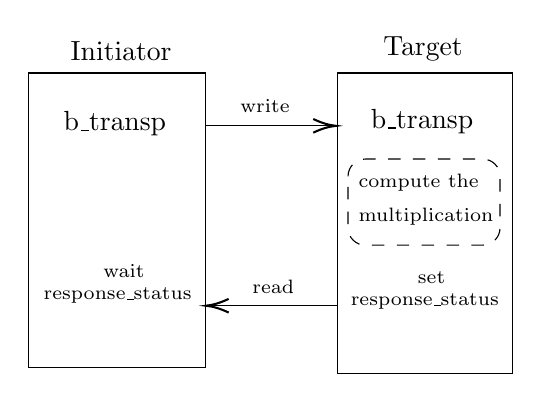
\begin{tikzpicture}[x=0.75pt,y=0.75pt,yscale=-1,xscale=1]
			%uncomment if require: \path (0,213); %set diagram left start at 0, and has height of 213
			
			%Shape: Rectangle [id:dp9211023518838333] 
			\draw   (5.25,26.54) -- (90.55,26.54) -- (90.55,168.28) -- (5.25,168.28) -- cycle ;
			%Rounded Rect [id:dp32759511217881776] 
			\draw  [dash pattern={on 4.5pt off 4.5pt}] (159.33,76.3) .. controls (159.33,71.71) and (163.05,68) .. (167.63,68) -- (224.25,68) .. controls (228.83,68) and (232.55,71.71) .. (232.55,76.3) -- (232.55,101.18) .. controls (232.55,105.76) and (228.83,109.48) .. (224.25,109.48) -- (167.63,109.48) .. controls (163.05,109.48) and (159.33,105.76) .. (159.33,101.18) -- cycle ;
			%Straight Lines [id:da5903625580084783] 
			\draw    (90.83,52) -- (151.51,52) ;
			\draw [shift={(153.51,52)}, rotate = 180] [color={rgb, 255:red, 0; green, 0; blue, 0 }  ][line width=0.75]    (10.93,-3.29) .. controls (6.95,-1.4) and (3.31,-0.3) .. (0,0) .. controls (3.31,0.3) and (6.95,1.4) .. (10.93,3.29)   ;
			
			%Straight Lines [id:da970665910373827] 
			\draw    (92.88,138.67) -- (154,138.67) ;
			
			\draw [shift={(90.88,138.67)}, rotate = 0] [color={rgb, 255:red, 0; green, 0; blue, 0 }  ][line width=0.75]    (10.93,-3.29) .. controls (6.95,-1.4) and (3.31,-0.3) .. (0,0) .. controls (3.31,0.3) and (6.95,1.4) .. (10.93,3.29)   ;
			%Shape: Rectangle [id:dp37760844118686276] 
			\draw   (154.25,26.54) -- (238.55,26.54) -- (238.55,171.48) -- (154.25,171.48) -- cycle ;
			
			% Text Node
			\draw (50,16) node   [align=left] {Initiator};
			% Text Node
			\draw (47,51) node   [align=left] {b\_transp};
			% Text Node
			\draw (196.88,87.52) node   [align=left] {{\scriptsize compute the}\\{\scriptsize multiplication}};
			% Text Node
			\draw (195.5,15) node   [align=left] {Target};
			% Text Node
			\draw (48.33,128.33) node  [font=\scriptsize] [align=left] { \ \ \ \ \ \ \ \ wait \\response\_status};
			% Text Node
			\draw (119.33,42.33) node  [font=\scriptsize] [align=left] {write};
			% Text Node
			\draw (195,50) node   [align=left] {b\_transp};
			% Text Node
			\draw (123.33,129.33) node  [font=\scriptsize] [align=left] {read};
			% Text Node
			\draw (196.33,131.33) node  [font=\scriptsize] [align=left] { \ \ \ \ \ \ \ \ \ set \\response\_status};
			
			
			\end{tikzpicture}
			\centering
			\caption{Schematic of the comunication at UT timing description.}
			\label{fig:utRappresentation}
		\end{figure}
		
	\begin{table}
		\begin{tabular}{@{}lllll@{}}
			\toprule
			Iterations & Real & User  & System \\ \midrule
			$10^3$   & 0,003s                    & 0,000s  & 0,003s \\
			$10^4$  & 0,021s                    & 0,000s    & 0,013s \\
			$10^5$ & 0,206s                    & 0,000s   & 0,146s \\
			$10^6$ & 2,203s                    & 0,016s   & 1,436s \\
			$10^7$ & 24,591s                    & 0,176s   & 16,320s \\
			$10^8$ & 4m 8,303s                    & 2,317s   & 2m 34,181s \\ 
			$10^9$ & 44m 30,274s             & 20,135s   & 27m 22,367s \\ \bottomrule
		\end{tabular}
		\centering
		\caption{UT simulation time results.}
		\label{UT simulation time results}
	\end{table}
	Each simulation, runned with the linux \verb|time| command, produces the values showed in Table ~\ref{UT simulation time results}. A plot of the values is showed on the Figure ~\ref{fig:utplot}.

	
	\begin{figure}

	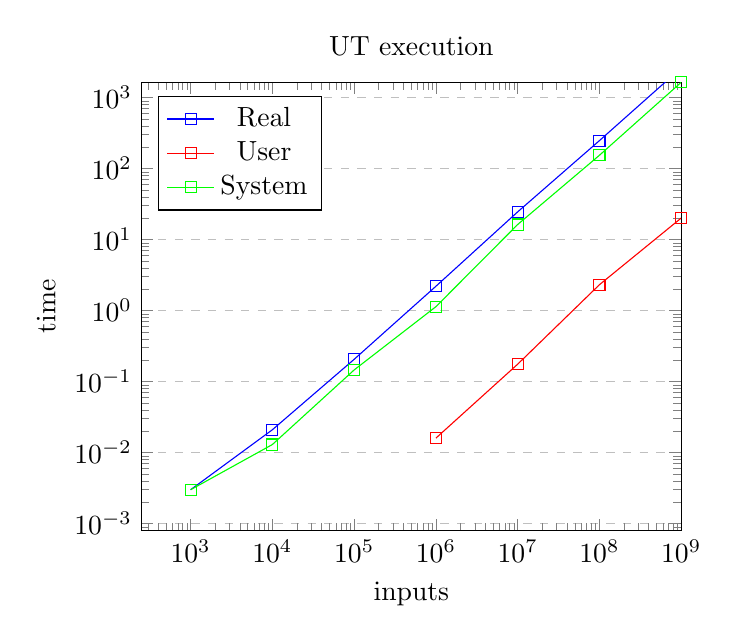
\begin{tikzpicture}
	\begin{axis}[
	title={UT execution},
	xlabel={inputs},
	ylabel={time},
	 xmax=1000000000,
ymax=1650,
xmode=log,
ymode=log,
	legend pos=north west,
	ymajorgrids=true,
	grid style=dashed,
	]
	
	\addplot[
	color=blue,
	mark=square,
	]
	coordinates {
		
		(1000, 0.003 )(10000, 0.021)(100000, 0.206 )(1000000, 2.203)(10000000, 24.591)(100000000, 248)(1000000000, 2618)
	};

	\addplot[
color=red,
mark=square,
]
coordinates {
	
	(1000, 0.0 )(10000, 0.0)(100000, 0.0 )(1000000, 0.016)(10000000, 0.176)(100000000, 2.317)(1000000000, 20.135)
};

	\addplot[
color=green,
mark=square,
]
coordinates {
	
	(1000, 0.003 )(10000, 0.013)(100000, 0.146 )(1000000, 1.136)(10000000, 16.320)(100000000, 154.181)(1000000000, 1642.367)
};

	\legend{Real, User, System}
	
	\end{axis}
	
	
	\end{tikzpicture}
	\centering
	\caption{Plot of the Table ~\ref{UT simulation time results} expressed in logaritmic scale.}
	\label{fig:utplot}
	
		\end{figure}
	
		
		
		
	\subsection{TLM: LT implementation}
	\label{sec:lt}
	The LT (\textit{loosely timed}) coding style, use blocking interface, and two synchronization points (which is invocation and return) and the temporal decoupling. This style allows a faster simulations than the RTL. The \verb|multiplier_LT_testbench| module, which is the initiator, use the \verb|b_transport| primitive as same as the UT implementation, but in this implementation we have the notion of $time$ for the synchronization: when the \verb|b_transport| primitive of the target (\verb|multiplier_LT|) is triggered, it create a \verb|SC_ZERO_TIME|  variable before the computation process, and on the $read$ phase, it pass back this variable to the initiator with the value of \verb|9ms| as expected timing for the computation. At this moment,  the initiator that waits for the target response, syncs the comunication if it is required, and resumes back to an another executions. The Figure ~\ref{fig:ltRappresentation} shows an abstract comunication between the two modules.
	The initiatior (which is the \textit{testbench}) calls the target different couples of time: from $10^3$ to $10^9$.
		Each simulation, produces the values showed in Table ~\ref{LT simulation time results}. A plot of the values is showed in the Figure ~\ref{ltplot}.
	
	
 	
 	\begin{figure}
 		
 		
 		\tikzset{every picture/.style={line width=0.75pt}} %set default line width to 0.75pt        
 		
 		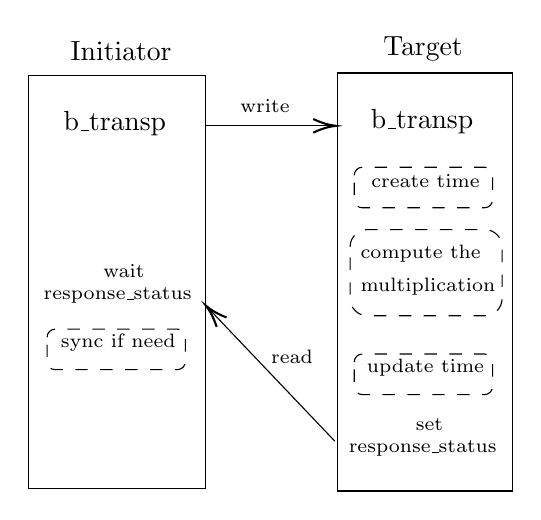
\begin{tikzpicture}[x=0.75pt,y=0.75pt,yscale=-1,xscale=1]
 		%uncomment if require: \path (0,426.14178466796875); %set diagram left start at 0, and has height of 426.14178466796875
 		
 		%Shape: Rectangle [id:dp9211023518838333] 
 		\draw   (5.25,27.54) -- (90.55,27.54) -- (90.55,226.93) -- (5.25,226.93) -- cycle ;
 		%Rounded Rect [id:dp32759511217881776] 
 		\draw  [dash pattern={on 4.5pt off 4.5pt}] (162.33,75.84) .. controls (162.33,73.68) and (164.08,71.93) .. (166.24,71.93) -- (225.06,71.93) .. controls (227.22,71.93) and (228.97,73.68) .. (228.97,75.84) -- (228.97,87.57) .. controls (228.97,89.73) and (227.22,91.48) .. (225.06,91.48) -- (166.24,91.48) .. controls (164.08,91.48) and (162.33,89.73) .. (162.33,87.57) -- cycle ;
 		%Straight Lines [id:da5903625580084783] 
 		\draw    (90.83,52) -- (151.51,52) ;
 		\draw [shift={(153.51,52)}, rotate = 180] [color={rgb, 255:red, 0; green, 0; blue, 0 }  ][line width=0.75]    (10.93,-3.29) .. controls (6.95,-1.4) and (3.31,-0.3) .. (0,0) .. controls (3.31,0.3) and (6.95,1.4) .. (10.93,3.29)   ;
 		
 		%Straight Lines [id:da970665910373827] 
 		\draw    (92.26,140.12) -- (152.97,203.93) ;
 		
 		\draw [shift={(90.88,138.67)}, rotate = 46.43] [color={rgb, 255:red, 0; green, 0; blue, 0 }  ][line width=0.75]    (10.93,-3.29) .. controls (6.95,-1.4) and (3.31,-0.3) .. (0,0) .. controls (3.31,0.3) and (6.95,1.4) .. (10.93,3.29)   ;
 		%Shape: Rectangle [id:dp37760844118686276] 
 		\draw   (154.25,26.54) -- (238.55,26.54) -- (238.55,227.93) -- (154.25,227.93) -- cycle ;
 		%Rounded Rect [id:dp20293607556805315] 
 		\draw  [dash pattern={on 4.5pt off 4.5pt}] (160.33,110.3) .. controls (160.33,105.71) and (164.05,102) .. (168.63,102) -- (225.25,102) .. controls (229.83,102) and (233.55,105.71) .. (233.55,110.3) -- (233.55,135.18) .. controls (233.55,139.76) and (229.83,143.48) .. (225.25,143.48) -- (168.63,143.48) .. controls (164.05,143.48) and (160.33,139.76) .. (160.33,135.18) -- cycle ;
 		%Rounded Rect [id:dp18525547874126558] 
 		\draw  [dash pattern={on 4.5pt off 4.5pt}] (162.33,165.84) .. controls (162.33,163.68) and (164.08,161.93) .. (166.24,161.93) -- (225.06,161.93) .. controls (227.22,161.93) and (228.97,163.68) .. (228.97,165.84) -- (228.97,177.57) .. controls (228.97,179.73) and (227.22,181.48) .. (225.06,181.48) -- (166.24,181.48) .. controls (164.08,181.48) and (162.33,179.73) .. (162.33,177.57) -- cycle ;
 		%Rounded Rect [id:dp07957647151925529] 
 		\draw  [dash pattern={on 4.5pt off 4.5pt}] (14.33,153.84) .. controls (14.33,151.68) and (16.08,149.93) .. (18.24,149.93) -- (77.06,149.93) .. controls (79.22,149.93) and (80.97,151.68) .. (80.97,153.84) -- (80.97,165.57) .. controls (80.97,167.73) and (79.22,169.48) .. (77.06,169.48) -- (18.24,169.48) .. controls (16.08,169.48) and (14.33,167.73) .. (14.33,165.57) -- cycle ;
 		
 		% Text Node
 		\draw (50,16) node   [align=left] {Initiator};
 		% Text Node
 		\draw (47,51) node   [align=left] {b\_transp};
 		% Text Node
 		\draw (196.65,78.7) node   [align=left] {{\scriptsize create time}};
 		% Text Node
 		\draw (195.5,15) node   [align=left] {Target};
 		% Text Node
 		\draw (48.33,128.33) node  [font=\scriptsize] [align=left] { \ \ \ \ \ \ \ \ wait \\response\_status};
 		% Text Node
 		\draw (119.33,42.33) node  [font=\scriptsize] [align=left] {write};
 		% Text Node
 		\draw (195,50) node   [align=left] {b\_transp};
 		% Text Node
 		\draw (132.33,163.33) node  [font=\scriptsize] [align=left] {read};
 		% Text Node
 		\draw (195.33,202.33) node  [font=\scriptsize] [align=left] { \ \ \ \ \ \ \ \ \ set \\response\_status};
 		% Text Node
 		\draw (197.88,121.52) node   [align=left] {{\scriptsize compute the}\\{\scriptsize multiplication}};
 		% Text Node
 		\draw (196.65,168.7) node   [align=left] {{\scriptsize update time}};
 		% Text Node
 		\draw (48.65,156.7) node   [align=left] {{\scriptsize sync if need}};
 		
 		
 		\end{tikzpicture}
			\centering
	\caption{Schematic of the comunication at LT timing description.}
	\label{fig:ltRappresentation}
	\end{figure}
 
 \begin{table}[]
 	\begin{tabular}{lllll}
 		\hline
			Iterations & Real & User  & System \\ \midrule
			$10^3$   & 0,004s                    & 0,000s  & 0,005s \\
			$10^4$  & 0,028s                    & 0,000s    & 0,023s \\
			$10^5$ & 0,266s                    & 0,000s   & 0,206s \\
			$10^6$ & 2,658s                    & 0,012s   & 1,888s \\
			$10^7$ & 27,591s                    & 0,325s   & 18,040s \\
			$10^8$ & 4m 43,521s                    & 3,510s   & 3m 2,549s \\ 
			$10^9$ & 47m 33,280s             & 33,321s   & 29m 39,531s \\ \bottomrule
 	\end{tabular}
 \centering
 \caption{LT simulation time results.}
 \label{LT simulation time results}
 \end{table}
	
		\begin{figure}

	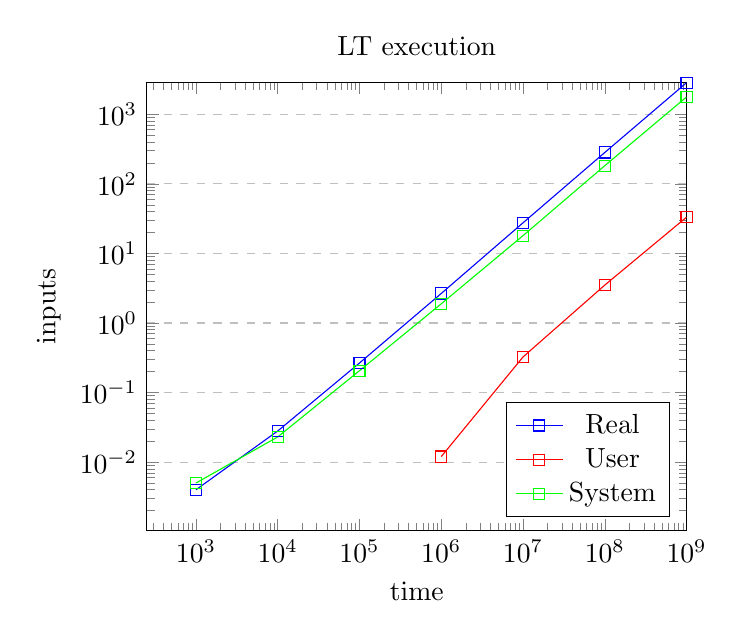
\begin{tikzpicture}
	\begin{axis}[
	title={LT execution},
	xlabel={time},
	ylabel={inputs},
	 xmax=1000000000,
ymax=2900,
xmode=log,
ymode=log,
	legend pos=south east,
	ymajorgrids=true,
	grid style=dashed,
	]

	\addplot[
color=blue,
mark=square,
]
coordinates {
	
	(1000, 0.004 )(10000, 0.028)(100000, 0.266 )(1000000, 2.658)(10000000, 27.591)(100000000, 283)(1000000000, 2853.280)
};

\addplot[
color=red,
mark=square,
]
coordinates {
	
	(1000, 0.0 )(10000, 0.0)(100000, 0.0 )(1000000, 0.012)(10000000, 0.325)(100000000, 3.510)(1000000000, 33.231)
};

\addplot[
color=green,
mark=square,
]
coordinates {
	
	(1000, 0.005 )(10000, 0.023)(100000, 0.206 )(1000000, 1.888)(10000000, 18.040)(100000000, 182.549)(1000000000, 1779.531)
};

\legend{Real, User, System}

	\end{axis}
	\end{tikzpicture}
	
				\centering
	\caption{Graph rappresentationf ot the Table ~\ref{LT simulation time results}}
	\label{ltplot}
\end{figure}

	\subsection{TLM: AT4 implementation}
\label{sec:at4}
The AT (\textit{approximately timed}) coding style, uses the non blocking interface provided from SystemC. The AT4 is a 4-phase handshaking protocol between the initiator and the target. This means that it will support a more detailed sequences of interactions between the two modules and makes the simulation similar of what happend on the RTL level. The non blocking transport interface, means that the module after the call of the transport primitive, instead of blocking it, will continue. 
The \verb|multiplier_LT_testbench| module, which is the initiator, use the \verb|nb_transport_fw| primitive to call the target, and then call the \verb|wait(event)| primitive to wait the target that send back the data on the \verb|nb_transport_bw| function when is ready.
On the other side, the target, when the \verb|nb_transport_fw| is triggered it calls the \verb|ioprocess()|, unlocked by the  \verb|notify(t_event)| primitive after the computation process. This create a callback to the initiator. 

\begin{figure}

\tikzset{every picture/.style={line width=0.75pt}} %set default line width to 0.75pt        

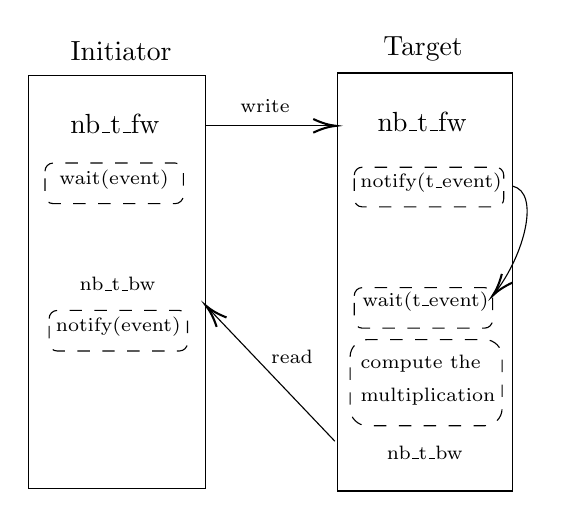
\begin{tikzpicture}[x=0.75pt,y=0.75pt,yscale=-1,xscale=1]
%uncomment if require: \path (0,257); %set diagram left start at 0, and has height of 257

%Shape: Rectangle [id:dp9211023518838333] 
\draw   (5.25,27.54) -- (90.55,27.54) -- (90.55,226.93) -- (5.25,226.93) -- cycle ;
%Rounded Rect [id:dp32759511217881776] 
\draw  [dash pattern={on 4.5pt off 4.5pt}] (162.33,75.75) .. controls (162.33,73.64) and (164.04,71.93) .. (166.15,71.93) -- (230.53,71.93) .. controls (232.64,71.93) and (234.35,73.64) .. (234.35,75.75) -- (234.35,87.22) .. controls (234.35,89.33) and (232.64,91.04) .. (230.53,91.04) -- (166.15,91.04) .. controls (164.04,91.04) and (162.33,89.33) .. (162.33,87.22) -- cycle ;
%Straight Lines [id:da5903625580084783] 
\draw    (90.83,52) -- (151.51,52) ;
\draw [shift={(153.51,52)}, rotate = 180] [color={rgb, 255:red, 0; green, 0; blue, 0 }  ][line width=0.75]    (10.93,-3.29) .. controls (6.95,-1.4) and (3.31,-0.3) .. (0,0) .. controls (3.31,0.3) and (6.95,1.4) .. (10.93,3.29)   ;

%Straight Lines [id:da970665910373827] 
\draw    (92.26,140.12) -- (152.97,203.93) ;

\draw [shift={(90.88,138.67)}, rotate = 46.43] [color={rgb, 255:red, 0; green, 0; blue, 0 }  ][line width=0.75]    (10.93,-3.29) .. controls (6.95,-1.4) and (3.31,-0.3) .. (0,0) .. controls (3.31,0.3) and (6.95,1.4) .. (10.93,3.29)   ;
%Shape: Rectangle [id:dp37760844118686276] 
\draw   (154.25,26.54) -- (238.55,26.54) -- (238.55,227.93) -- (154.25,227.93) -- cycle ;
%Rounded Rect [id:dp20293607556805315] 
\draw  [dash pattern={on 4.5pt off 4.5pt}] (160.33,163.3) .. controls (160.33,158.71) and (164.05,155) .. (168.63,155) -- (225.25,155) .. controls (229.83,155) and (233.55,158.71) .. (233.55,163.3) -- (233.55,188.18) .. controls (233.55,192.76) and (229.83,196.48) .. (225.25,196.48) -- (168.63,196.48) .. controls (164.05,196.48) and (160.33,192.76) .. (160.33,188.18) -- cycle ;
%Rounded Rect [id:dp18525547874126558] 
\draw  [dash pattern={on 4.5pt off 4.5pt}] (162.33,133.84) .. controls (162.33,131.68) and (164.08,129.93) .. (166.24,129.93) -- (225.06,129.93) .. controls (227.22,129.93) and (228.97,131.68) .. (228.97,133.84) -- (228.97,145.57) .. controls (228.97,147.73) and (227.22,149.48) .. (225.06,149.48) -- (166.24,149.48) .. controls (164.08,149.48) and (162.33,147.73) .. (162.33,145.57) -- cycle ;
%Rounded Rect [id:dp07957647151925529] 
\draw  [dash pattern={on 4.5pt off 4.5pt}] (13.33,73.84) .. controls (13.33,71.68) and (15.08,69.93) .. (17.24,69.93) -- (76.06,69.93) .. controls (78.22,69.93) and (79.97,71.68) .. (79.97,73.84) -- (79.97,85.57) .. controls (79.97,87.73) and (78.22,89.48) .. (76.06,89.48) -- (17.24,89.48) .. controls (15.08,89.48) and (13.33,87.73) .. (13.33,85.57) -- cycle ;
%Rounded Rect [id:dp640167309122506] 
\draw  [dash pattern={on 4.5pt off 4.5pt}] (15.33,144.84) .. controls (15.33,142.68) and (17.08,140.93) .. (19.24,140.93) -- (78.06,140.93) .. controls (80.22,140.93) and (81.97,142.68) .. (81.97,144.84) -- (81.97,156.57) .. controls (81.97,158.73) and (80.22,160.48) .. (78.06,160.48) -- (19.24,160.48) .. controls (17.08,160.48) and (15.33,158.73) .. (15.33,156.57) -- cycle ;
%Curve Lines [id:da29853654644367633] 
\draw    (238.5,81) .. controls (252.15,83.93) and (244.38,114.27) .. (230.08,132.47) ;
\draw [shift={(228.97,133.84)}, rotate = 309.81] [color={rgb, 255:red, 0; green, 0; blue, 0 }  ][line width=0.75]    (10.93,-3.29) .. controls (6.95,-1.4) and (3.31,-0.3) .. (0,0) .. controls (3.31,0.3) and (6.95,1.4) .. (10.93,3.29)   ;


% Text Node
\draw (50,16) node   [align=left] {Initiator};
% Text Node
\draw (47,51) node   [align=left] {nb\_t\_fw};
% Text Node
\draw (199.34,79.48) node   [align=left] {{\scriptsize notify(t\_event)}};
% Text Node
\draw (195.5,15) node   [align=left] {Target};
% Text Node
\draw (48.33,128.33) node  [font=\scriptsize] [align=left] {nb\_t\_bw};
% Text Node
\draw (119.33,42.33) node  [font=\scriptsize] [align=left] {write};
% Text Node
\draw (195,50) node   [align=left] {nb\_t\_fw};
% Text Node
\draw (132.33,163.33) node  [font=\scriptsize] [align=left] {read};
% Text Node
\draw (196.33,209.33) node  [font=\scriptsize] [align=left] {nb\_t\_bw};
% Text Node
\draw (197.88,174.52) node   [align=left] {{\scriptsize compute the}\\{\scriptsize multiplication}};
% Text Node
\draw (196.65,136.7) node   [align=left] {{\scriptsize wait(t\_event)}};
% Text Node
\draw (46.65,77.7) node   [align=left] {{\scriptsize wait(event)}};
% Text Node
\draw (48.65,148.7) node   [align=left] {{\scriptsize notify(event)}};

 		
\end{tikzpicture}
\centering
\caption{Schematic of the comunication at AT4 timing description.}
\label{fig:at4Rappresentation}
\end{figure}


 
\begin{table}[]
	\begin{tabular}{lllll}
		\hline
		Iterations & Real & User  & System \\ \midrule
		$10^3$   & 0,004s                    & 0,000s  & 0,004s \\
		$10^4$  & 0,029s                    & 0,000s    & 0,029s \\
		$10^5$ & 0,323s                    & 0,000s   & 0,287s \\
		$10^6$ & 3,456s                    & 0,052s   & 2,768s \\
		$10^7$ & 35,571s                    & 0,558s   & 27,637s \\
		$10^8$ & 5m 54,022s                    & 7,184s   & 4m 21,377s \\ 
		$10^9$ & 61m 0,820s             & 1m 20,609s   & 44m 25,017s \\ \bottomrule
	\end{tabular}
	\centering
	\caption{AT4 simulation time results.}
	\label{AT4 simulation time results}
\end{table}

The Figure ~\ref{fig:at4Rappresentation} shows an abstract comunication between the two modules.
The initiatior (which is the \textit{testbench}) call the target different couples of time: from $10^3$ to $10^9$.

	\begin{figure}
	
	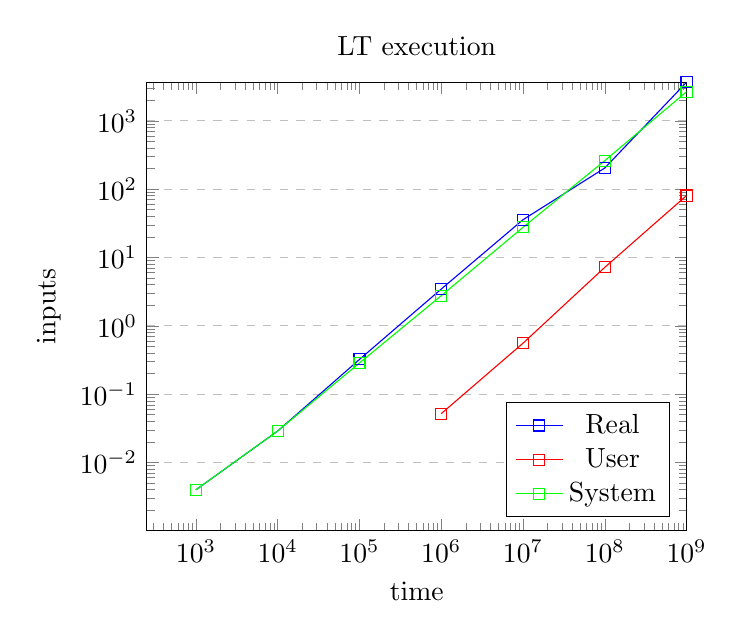
\begin{tikzpicture}
	\begin{axis}[
	title={LT execution},
	xlabel={time},
	ylabel={inputs},
	xmax=1000000000,
	ymax=3670,
	xmode=log,
	ymode=log,
	legend pos=south east,
	ymajorgrids=true,
	grid style=dashed,
	]
	
	\addplot[
	color=blue,
	mark=square,
	]
	coordinates {
		
		(1000, 0.004 )(10000, 0.029)(100000, 0.323 )(1000000, 3.456)(10000000, 35.71)(100000000, 204.002)(1000000000, 3660.820)
	};
	
	\addplot[
	color=red,
	mark=square,
	]
	coordinates {
		
		(1000, 0.0 )(10000, 0.0)(100000, 0.0 )(1000000, 0.052)(10000000, 0.558)(100000000, 7.184)(1000000000, 80.609)
	};
	
	\addplot[
	color=green,
	mark=square,
	]
	coordinates {
		
		(1000, 0.004 )(10000, 0.029)(100000, 0.287 )(1000000, 2.768)(10000000, 27.637)(100000000, 261.377)(1000000000, 2665)
	};
	
	\legend{Real, User, System}
	
	\end{axis}
	\end{tikzpicture}
	
	\centering
	\caption{Plot of the Table ~\ref{LT simulation time results} expressed in logaritmic scale.}
	\label{ltplot}
\end{figure}

Each simulation produces the values showed in Table ~\ref{AT4 simulation time results}. A plot of the values is showed in the Figure ~\ref{ltplot}.


\begin{table}[]
	\begin{tabular}{lllll}
		\hline
		Iterations & Real & User  & System \\ \midrule
		$10^3$   & 0,045s                    & 0,005s  & 0,041s \\
		$10^4$  & 0,430s                    & 0,080s    & 0,350 \\
		$10^5$ & 4,147s                    & 0,256s   & 3,890s \\
		$10^6$ & 39,069s                    & 3,732s   & 35,337s \\
		$10^7$ & 6m 33,900s                    & 33,844s   & 5m 59,745s \\
			$10^8$ & 65m 52,598s                    & 5m 22,510s   & 60m 30,056s \\ 
		$10^9$ & 716m 38,452s           & 45m 42,970  & 670m 54,149s \\ \bottomrule
	\end{tabular}
	\centering
	\caption{RTL simulation time results.}
	\label{RTL simulation time results}
\end{table}
	\begin{figure}
	
	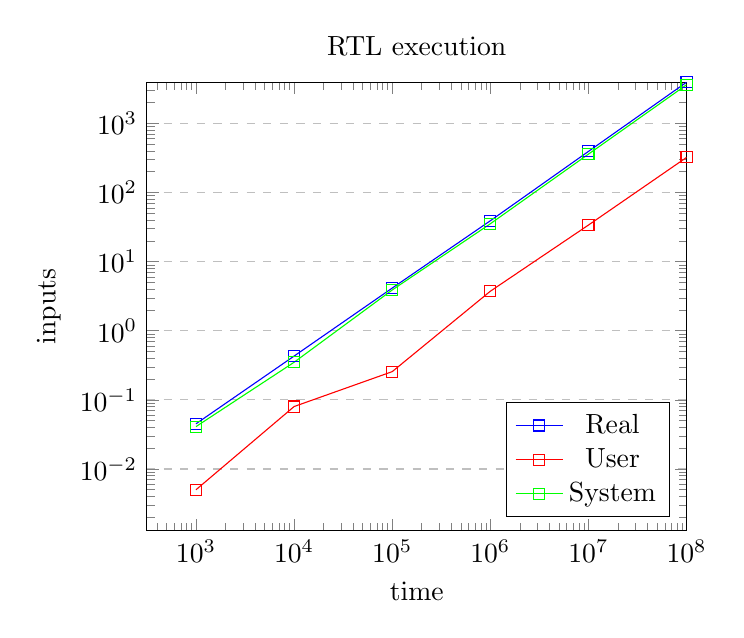
\begin{tikzpicture}
	\begin{axis}[
	title={RTL execution},
	xlabel={time},
	ylabel={inputs},
	xmax=100000000,
	ymax=3955,
	xmode=log,
	ymode=log,
	legend pos=south east,
	ymajorgrids=true,
	grid style=dashed,
	]
	
	\addplot[
	color=blue,
	mark=square,
	]
	coordinates {
		
		(1000, 0.045 )(10000, 0.430)(100000, 4.147 )(1000000, 39.069)(10000000, 393.900)(100000000, 3952.598)
	};
	
	\addplot[
	color=red,
	mark=square,
	]
	coordinates {
		
		(1000, 0.005 )(10000, 0.080)(100000, 0.256 )(1000000, 3.732)(10000000, 33.844)(100000000, 322.510)
	};
	
	\addplot[
	color=green,
	mark=square,
	]
	coordinates {
		
	
	(1000, 0.041 )(10000, 0.350)(100000, 3.890 )(1000000, 35.337)(10000000, 359.745)(100000000, 3630.056)
	};
	
	\legend{Real, User, System}
	
	\end{axis}
	\end{tikzpicture}
	
	\centering
	\caption{Plot of the Table ~\ref{RTL simulation time results} expressed in logaritmic scale.}
	\label{rtlplot}
\end{figure}


	\subsection{TLM: RTL implementation}
	\label{sec:rtlimpl}
	The SystemC-RTL implementation of the IEE754 multiplier, described in details on the previous report, it is tested with the same simulation of UT, LT and AT4, producing the values reported on the Table ~\ref{RTL simulation time results}.


	\begin{figure}
	
	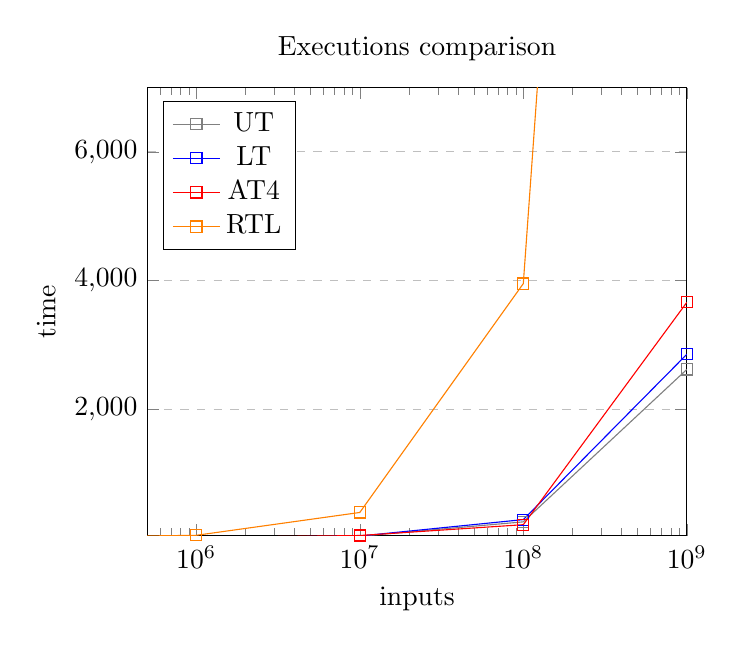
\begin{tikzpicture}
	\begin{axis}[
	title={Executions comparison},
	xlabel={inputs},
	ylabel={time},
	 ymin=30,
	 xmode=log,
	xmax=1000000000,
	ymax=7000,
	legend pos=north west,
	ymajorgrids=true,
	grid style=dashed,
	]
	
	\addplot[
color=gray,
mark=square,
]
coordinates {
	
	(1000, 0.003 )(10000, 0.021)(100000, 0.206 )(1000000, 2.203)(10000000, 24.591)(100000000, 248)(1000000000, 2618)
};


	\addplot[
color=blue,
mark=square,
]
coordinates {
	
	(1000, 0.004 )(10000, 0.028)(100000, 0.266 )(1000000, 2.658)(10000000, 27.591)(100000000, 283)(1000000000, 2853.280)
};

	
\addplot[
color=red,
mark=square,
]
coordinates {
	
	(1000, 0.004 )(10000, 0.029)(100000, 0.323 )(1000000, 3.456)(10000000, 35.71)(100000000, 204.002)(1000000000, 3660.820)
};

	
\addplot[
color=orange,
mark=square,
]
coordinates {
	
	(1000, 0.045 )(10000, 0.430)(100000, 4.147 )(1000000, 39.069)(10000000, 393.900)(100000000, 3952.598)
	(1000000000, 39520.598)
};

	\legend{UT, LT, AT4, RTL}
	
	\end{axis}
	
	
	\end{tikzpicture}
	\centering
	\caption{Plot of the different 'Real' time annotation with all TLM code styles.}
	\label{fig:diffplot}
	
\end{figure}



\subsection{TLM:  report}
\label{sec:ltmreport}
From the previous sections, is possible to view how the simulation time change from the UT to the RTL. The Figure ~\ref{fig:diffplot} displays the differences between the UT, LT, AT4 and RTL. The AT4 description, having a better description of the specification, and a detailed handshake protocol for the comunication between the target and initiator, it wil decrease the simulation speed compared with UT. But the greater detachment is shown with the simulation of $10^9$ cycles by RTL. 
The system simulation time changed from 44m for UT up to 716m ($ca.$12h) for RTL. This means that in TLM, is optimal for simulation with and abstract description respect the RTL level, and with that information, we have to take care of the relationship between the module refining and the simulation speed when we are working on the hardware design.

The Figures [~\ref{fig:ut-cpu}, ~\ref{fig:lt-cpu}, ~\ref{fig:at4-cpu}, ~\ref{fig:rtl-cpu}] show the CPU and memory usage during each simulation.

\section{Virtual Platform Integration}
\label{sec:vp}
The virtual platform used in this project, showed in Figure ~\ref{fig:vpRappresentation}, is composed by a CPU MOS 6502 (1976), with 16bit addressing and 8bit data width, a Memory block composed by ROM, RAM and clock divided (for manage the MIMO operations and memory), a APB ARM BUS, which supports 8 peripherals, and an I/O Moduled which is used for I/O from/to the platform.

\subsection{VP: Integration}
\label{sec:vpintegration}
This VP allows to load a cross-compiled software and run a software with the I/O integration. Is choosed not to connect the IEEE754 multiplicator top level created on the previous report, but to connect directly the two  VHDL and Verilog IEEE754 multiplicator as peripheral on the platform. 

This choice was determined by the fact that it was wanted to test the VHDL and Verilog multipliers independently as if they were two slaves connected to the AMBA BUS, firstly checking that the VP is working with more peripheral connected, and then use on the other side of the AMBA BUS, the cross-compiled software with new routines and main function that give to the multipliers the same or different inputs, using the I/O module to verify that the result obtained from them is correct or not. 

During the integretion one must take care to the clock of the platform: the multipliers are working with a 32bit data, but the CPU and Memory communicate with a 8bit. This means that the clock speed of the CPU is 4 times faster than the clock of the multiplier.

This kind of implementation described above can be confusing for a moment, so let's explain step by step the integration flow:

\subsection{VP: Cross-compiled software}
\label{sec:vpprjstructure}
The project structure is shown on the follow directory tree:
	\\
\begin{forest}
	for tree={
		font=\ttfamily,
		grow'=0,
		child anchor=west,
		parent anchor=south,
		anchor=west,
		calign=first,
		edge path={
			\noexpand\path [draw, \forestoption{edge}]
			(!u.south west) +(7.5pt,0) |- node[fill,inner sep=1.05pt] {} (.child anchor)\forestoption{edge label};
		},
		before typesetting nodes={
			if n=1
			{insert before={[,phantom]}}
			{}
		},
		fit=band,
		before computing xy={l=13pt},
	}
	[root (splatters)
	[application]
	[platform]
	[cc65]
	]
\end{forest}
\\
The \verb|application| folder contains the sources of the cross-compiled software. \verb|platform| contains the Vivado project (with the .v and .vhdl sources), used for simulation.  \verb|cc65| contains the compiler.
\\
Because is chosen to link two multipliers on the VP, two routines was added on the cross-compiled software in \verb|routines.c|: one for the verilog multiplier, and one for the VHDL multiplier. The Verilog is connected to the peripheral 3, and the VHDL at the 4. The two routines, accept as parameter the two operand having \verb|uint32_t| as type. The VHDL routine is showed below:
\\
\\
\noindent
\begin{minipage}{.45\textwidth}
	\begin{lstlisting}[,frame=tlrb]{Name}
reset_flags();
set_pwdata(op1);
set_psel(PSEL4);
set_penable(1);

set_penable(0);
set_pwdata(op2);
set_psel(PSEL4);
set_penable(1);

while (get_pready() == 0)
   __asm__("nop");

result = get_prdata();
set_penable(0);
set_psel(NO_PSEL);

	\end{lstlisting}
\end{minipage}\hfill
The \verb|main.c| file is changed to work as testbench, using the I/O module to read and write the data:
\\
\\
\noindent
\begin{minipage}{.45\textwidth}
	\begin{lstlisting}[,frame=tlrb]{Name}
[...]
test_mul_verilog(op1, op2, &res1);
test_mul_vhdl(op1, op2, &res2);
if (res1 == res2) {
  io_write(1);
} else {
  io_write(0);
}
equals = io_read();
[...]
	\end{lstlisting}
\end{minipage}\hfill
The main function calls the two multiplier routines, passing the same data as input. When the multipliers finish the computations, if the data obtained  (\verb|res1| and  \verb|res2|) are equals, it means that the two multipliers work and the software write with the I/O module the value of  \verb|1|.
The routines previously created, anticipate the way of how our multipliers communicate with the VP showed on the next section.
\subsection{VP: multiplier wrapping}
\label{sec:vphdlwrap}
After the creation of the routines, the multipliers are wrapped to the VP (now working inside the \verb|platform| folder).
Is not possible to connect directly the two multipliers to the AMBA BUS, because the multipliers and the AMBA BUS have different signals and  protocols of comunication. So it was created an APB Wrapper for each multiplier: one in Verilog, and one in VHDL.

The wrapper has two functions: the first one is to communicate with the AMBA BUS, and the second one is to run as toplevel for the multiplier IEEE754 module. The Figure ~\ref{fig:apbwrapper} shows a schematic of our peripheral connection.

The APB wrapper component (which is the toplevel for the multiplier module) works as an EFSM, showed in Figure ~\ref{fig:wrappertoplevel} and it has 5 states. The protocol works like that:
\begin{itemize}
	\item The \verb|presetn| works as reset value.
	\item When the \verb|penable| signal recieved from APB, has the value of \verb|1|, it tells to the toplevel when the first operand is ready, and it is saved on a \verb|tmp| signal at the state \verb|ST_1|.
	\item When the \verb|penable| now switches to \verb|0| moves the FSM to the state \verb|ST_2|. When it returns back to \verb|1| it means that the second operand is ready and moves the FSM to the state \verb|ST_3|. At this time the toplevel sets the \verb|in_rdy| with value of \verb|1| to make the nested multiplier module start to compute the multiplication.
	\item Now it waits until the \verb|res_rdy| signal of multiplier is setted as \verb|1|, to move on the FSM at the state \verb|ST_4| and set the \verb|prdata| signal with the result (and also \verb|pready| for tell the data is ready).
\end{itemize}
So, the APB Wrapper comunication protocol uses the \verb|penable| signal for handle the first and the second operand for the multiplier module. A sequence diagram of the protocol, with the comunication between master and slave is showed in Figure~\ref{fig:seqDiagram}.

Some modifications to the toplevel and testbench of the platofm are required to integrate the multiplier and the APB wrapper. 

On the \verb|top_level.v| file were added the wires to handle the data binding for the two new peripheral deivces (previus Verilog and VHDL multipliers wrappers), where $'X'$ stands for the peripheral number:
\\
\\
\noindent
\begin{minipage}{.45\textwidth}
	\begin{lstlisting}[,frame=tlrb]{Name}
wire  apb_X_pclk;
wire  apb_X_presetn;
wire  apb_X_psel;
wire  apb_X_penable;
wire  apb_X_pwrite;
wire  apb_X_pready;
wire  [31:0] apb_X_pwdata;
wire  [31:0] apb_X_paddr;
wire  [31:0] apb_X_prdata;
	\end{lstlisting}
\end{minipage}\hfill
Now this signals were mapped to the \verb|amba_apb_bus| as follow:
\\
\\
\noindent
\begin{minipage}{.45\textwidth}
	\begin{lstlisting}[,frame=tlrb]{Name}
 amba_apb_bus bus(  
 	.clk(clk_div4),
	.apb_master_presetn(presetn),
	[...]
	.apb_X_pclk(apb_X_pclk),
	.apb_X_presetn(apb_X_presetn),
	.apb_X_paddr(apb_X_paddr),
	.apb_X_psel(apb_X_psel),
	.apb_X_penable(apb_X_penable),
	.apb_X_pwrite(apb_X_pwrite),
	.apb_X_pwdata(apb_X_pwdata),
	.apb_X_pready(apb_X_pready),
	.apb_X_prdata(apb_X_prdata),
	[...]
    );
	\end{lstlisting}
\end{minipage}\hfill
Then the signals are mapped to the APB wrapper. The Verilog APB wrapper is reported below:
\\
\\
\noindent
\begin{minipage}{.45\textwidth}
	\begin{lstlisting}[,frame=tlrb]{Name}
mul_verilog_apb_wrapper mul_v(  
	.pclk(apb_3_pclk),
	.presetn(apb_3_presetn),
	.paddr(apb_3_paddr),
	.psel(apb_3_psel),
	.penable(apb_3_penable),
	.pwrite(apb_3_pwrite),  
	.pwdata(apb_3_pwdata),
	.pready(apb_3_pready),
	.prdata(apb_3_prdata));
	\end{lstlisting}
\end{minipage}\hfill
That's all. Now the multiplier wrapper is connected to the AMBA BUS, and is able to receive the signals and command previously created on the cross-compiled software (inside the \textit{routines.c}). Even if in the cross-compiled software we make the check for the multiplier correctness that write the value of \verb|1| if the results are the same, on the \verb|tb.v| file we check that the I/O module is writing on it.
For that, this row were added on the \verb|tb.v| that prints the value writed on I/O module from the software, displayed on the Vivado tlc console:
\\
\\
\noindent
\begin{minipage}{.45\textwidth}
	\begin{lstlisting}[,frame=tlrb]{Name}
while(~dout_rdy)begin #20; end
$display("Out: %d ", dout);
	\end{lstlisting}
\end{minipage}\hfill
The Table ~\ref{vpmapping} shows how the signals are mapped togheder in the platform. The next section will report the simulation of the VP.

\begin{table}[]
\begin{tabular}{@{}lllll@{}}
	\toprule
	\multicolumn{2}{c}{APB BUS} & \multicolumn{1}{c}{Top Level} & \multicolumn{1}{c}{Wrapper} & \multicolumn{1}{c}{Multiplier} \\ \midrule
	& apb\_X\_pclk        & apb\_X\_pclk                  & pclk                        & used (mapped to clk)           \\
	& apb\_X\_presetn     & apb\_X\_presetn               & presetn                     & used (mapped to rst)           \\
	& apb\_X\_paddr       & apb\_X\_paddr                 & paddr                       & not used                       \\
	& apb\_X\_psel        & apb\_X\_psel                  & psel                        & not used                       \\
	& apb\_X\_penable     & apb\_X\_penable               & penable                     & used                           \\
	& apb\_X\_pwrite      & apb\_X\_pwrite                & pwrite                      & not used                       \\
	& apb\_X\_pwdata      & apb\_X\_pwdata                & pwdata                      & used (mapped to op1, op2)      \\
	& apb\_X\_pready      & apb\_X\_pready                & pready                      & used                           \\
	& apb\_X\_prdata      & apb\_X\_prdata                & prdata                      & used (mapped to res)           \\ \bottomrule
\end{tabular}
	\centering
	\caption{VP signals mapping between modules.}
	\label{vpmapping}
\end{table}


\begin{figure}
\tikzset{every picture/.style={line width=0.75pt}} %set default line width to 0.75pt        

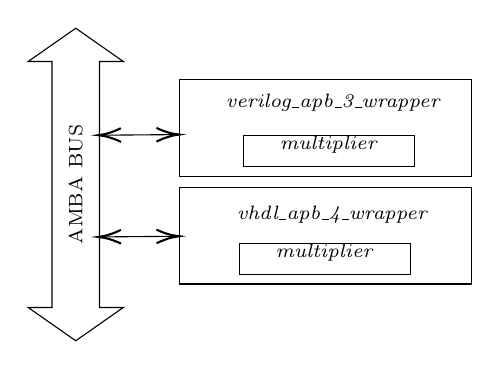
\begin{tikzpicture}[x=0.75pt,y=0.75pt,yscale=-1,xscale=1]
%uncomment if require: \path (0,345.3104705810547); %set diagram left start at 0, and has height of 345.3104705810547

%Up Down Arrow [id:dp2817398494023984] 
\draw   (7.48,20.79) -- (30.38,4.77) -- (53.27,20.79) -- (41.82,20.79) -- (41.82,139.33) -- (53.27,139.33) -- (30.38,155.35) -- (7.48,139.33) -- (18.93,139.33) -- (18.93,20.79) -- cycle ;
%Shape: Rectangle [id:dp6949852059810868] 
\draw   (80.4,29.54) -- (221.2,29.54) -- (221.2,76) -- (80.4,76) -- cycle ;
%Shape: Rectangle [id:dp8955494647270708] 
\draw   (80.4,81.54) -- (221.2,81.54) -- (221.2,128) -- (80.4,128) -- cycle ;
%Straight Lines [id:da6466953946936234] 
\draw    (78.2,56.02) -- (43.2,56.31) ;
\draw [shift={(41.2,56.32)}, rotate = 359.52] [color={rgb, 255:red, 0; green, 0; blue, 0 }  ][line width=0.75]    (10.93,-3.29) .. controls (6.95,-1.4) and (3.31,-0.3) .. (0,0) .. controls (3.31,0.3) and (6.95,1.4) .. (10.93,3.29)   ;
\draw [shift={(80.2,56)}, rotate = 179.52] [color={rgb, 255:red, 0; green, 0; blue, 0 }  ][line width=0.75]    (10.93,-3.29) .. controls (6.95,-1.4) and (3.31,-0.3) .. (0,0) .. controls (3.31,0.3) and (6.95,1.4) .. (10.93,3.29)   ;
%Straight Lines [id:da6950140444976091] 
\draw    (78.2,105.02) -- (43.2,105.31) ;
\draw [shift={(41.2,105.32)}, rotate = 359.52] [color={rgb, 255:red, 0; green, 0; blue, 0 }  ][line width=0.75]    (10.93,-3.29) .. controls (6.95,-1.4) and (3.31,-0.3) .. (0,0) .. controls (3.31,0.3) and (6.95,1.4) .. (10.93,3.29)   ;
\draw [shift={(80.2,105)}, rotate = 179.52] [color={rgb, 255:red, 0; green, 0; blue, 0 }  ][line width=0.75]    (10.93,-3.29) .. controls (6.95,-1.4) and (3.31,-0.3) .. (0,0) .. controls (3.31,0.3) and (6.95,1.4) .. (10.93,3.29)   ;
%Shape: Rectangle [id:dp9061085629462738] 
\draw   (109.4,108.54) -- (191.58,108.54) -- (191.58,123.35) -- (109.4,123.35) -- cycle ;
%Shape: Rectangle [id:dp1976757693153366] 
\draw   (111.4,56.54) -- (193.58,56.54) -- (193.58,71.35) -- (111.4,71.35) -- cycle ;

% Text Node
\draw (30.38,80.06) node  [rotate=-270.01] [align=left] {{\scriptsize AMBA BUS}};
% Text Node
\draw (154.65,40.7) node   [align=left] {{\scriptsize \textit{verilog\_apb\_3\_wrapper}}};
% Text Node
\draw (154.27,94.7) node   [align=left] {{\scriptsize \textit{vhdl\_apb\_4\_wrapper}}};
% Text Node
\draw (150.49,112.94) node   [align=left] {{\scriptsize \textit{multiplier}}};
% Text Node
\draw (152.49,60.94) node   [align=left] {{\scriptsize \textit{multiplier}}};


\end{tikzpicture}
\centering
\caption{APB wrapper schema}
\label{fig:apbwrapper}
\end{figure}

\subsection{VP: simulation}
\label{sec:vphdlwrap}
For simulating the platform, firstly the software is cross-compiled with the cc65, that produces a \verb|rom.mem| file which is imported in Vivado as a simulation source. Then the simulation was run. 
The value of op1 is 3 (\textit{hex: 0x40400000}) and the value of op2 is 2 (\textit{hex: 0x40000000}), expecting 6 (\textit{hex: 0x40c00000}) as result.
\\

The Figure ~\ref{fig:verilog} displays the waveforms of the simulation for the peripherical number 3, which is the verilog APB wrapper module. As we can see, on row 18 there is the \verb|psel| signal which indicate that the peripheral is selected, then at row 19 there is the \verb|penable| signal, and its change from value of 0 to 1 determines the state changes of the FSM of the wrapper that can be viewed at row 25. The vertical marker (\textit{yellow}) shows the time where the peripherical start moving on the FSM excuting its process. 
The Figure ~\ref{fig:verilogzoom} report a \textit{zoom-in} when the APB wrapper is ready to return back the result, that can be viewed at row 29. Even if at the row 29 is difficult to see the result obtained from the multiplier, at the row 23 the \verb|prdata| assume the value of \textit{0x40c00000} which is our correct result!

Another thing that can be see from the Figure ~\ref{fig:verilogzoom} its the difference from the \verb|pclk| of the APB wrapper (row 15) and the clk of the CPU (row 1): the CPU clock is 4 times faster of the APB wrapper. This cause the delay between the first time the  \verb|penable|  goes up to 1 and the second time for transfer the data.
\\

The vhdl wrapper simulation is the same as the one already observed; The Figure ~\ref{fig:verilogbinding} shows the waveforms and correctness of the binding signals between the AMBA BUS and the APB wrapper. Meanwhile the Figure ~\ref{fig:longsimulation} displays an entire simulation with the most important signals.

Finally, after the execution of the simulation, on the tlc console is possible to view that the cross-compiled software checks correctly the multiplier result and writes the check valus on the IO module readed on the testbench:
\\
\\
\noindent
\begin{minipage}{.45\textwidth}
	\begin{lstlisting}[,frame=tlrb]{Name}
restart
run 2ms
Out:  1 
	\end{lstlisting}
\end{minipage}\hfill
Where 1 means that its multiplication results is correct.

	\section{Conclusion}
	The table on the right speaks for itself: SystemC simulation is optimal for time to market, co-design and model verification, improving with the virtual platforms the possibility to reuse IPs and/or integrate new ones already existing, but you can easily notice from the data obtained that a description at TLM or RTL level changes considerably the simulation time.
	The choice to describe the operation of the HW component through LT or AT transitions is a choice of the level of refinement you want to go on: in the case that you choose a minor detail and a simulation closer to the RTL, but you don't want to simulate at RTL level, or you don't have the RTL description, through SystemC-TLM and AT (AT4) style you can find a good compromise between development speed, simulation and verification compared to a module described at RTL level with an HDL language.
	
	\bibliographystyle{IEEEtran}
	\bibliography{biblio}

\newpage
\begin{sidewaystable} 
	\begin{tabular}{@{}lllllllllllll@{}}
		\toprule
		Values                          & \multicolumn{4}{c}{Real}                                                  & \multicolumn{4}{c}{User}                                      & \multicolumn{4}{c}{System}                                         \\ \midrule
		\multicolumn{1}{l|}{}           & UT          & LT          & AT4         & \multicolumn{1}{l|}{RTL}        & UT      & LT      & AT4        & \multicolumn{1}{l|}{RTL}     & UT          & LT          & AT4         & \multicolumn{1}{l|}{RTL} \\ \cmidrule(l){2-13} 
		\multicolumn{1}{l|}{$10^3$}       & 0,003s      & 0,004s      & 0,004s      & \multicolumn{1}{l|}{0,045s}     & 0,000s  & 0,000s  & 0,000s     & \multicolumn{1}{l|}{0,005s}  & 0,003s      & 0,005s      & 0,004s      & 0,041s                   \\
		\multicolumn{1}{l|}{$10^4$}      & 0,021s      & 0,028s      & 0,029s      & \multicolumn{1}{l|}{0,430s}     & 0,000s  & 0,000s  & 0,000s     & \multicolumn{1}{l|}{0,080s}  & 0,013s      & 0,023s      & 0,029s      & 0,350s                   \\
		\multicolumn{1}{l|}{$10^5$}     & 0,206s      & 0,266s      & 0,323s      & \multicolumn{1}{l|}{4,147s}     & 0,000s  & 0,000s  & 0,000s     & \multicolumn{1}{l|}{0,256s}  & 0,146s      & 0,206s      & 0,287s      & 3,890                   \\
		\multicolumn{1}{l|}{$10^6$}    & 2,203s      & 2,658s      & 3,456s      & \multicolumn{1}{l|}{39,069s}    & 0,016s  & 0,012s  & 0,052s     & \multicolumn{1}{l|}{3,732s}  & 1,436s      & 1,888s      & 2,768s      & 35,337s               \\
		\multicolumn{1}{l|}{$10^7$}   & 24,591s     & 27,591s     & 35,571s     & \multicolumn{1}{l|}{6m 33,9s} & 0,176s  & 0,325s  & 0,558s     & \multicolumn{1}{l|}{33,844s} & 16,320s     & 18,040s     & 27,637s     &               5m 59,7s           \\
		\multicolumn{1}{l|}{$10^8$}  & 4m 8,3s   & 4m 43,5s  & 5m 54,0s  & \multicolumn{1}{l|}{65m 52,5s}           & 2,317s  & 3,510s  & 7,184s     & \multicolumn{1}{l|}{5m 22,5s}        & 2m 34,1s  & 3m 2,5s   & 4m 21,3s  &    60m 30,0s                      \\
		\multicolumn{1}{l|}{$10^9$} & 44m 30,2s & 47m 33,2s & 61m 0,8s & \multicolumn{1}{l|}{716m 38s}           & 20,135s & 33,321s & 1m 20,6s & \multicolumn{1}{l|}{45m 42s}        & 27m 22,3s & 29m 39,5s & 44m 25,0s & 670m 54s\\ \bottomrule
	\end{tabular}
\end{sidewaystable}



		\newpage




\begin{figure*}[ht]
\tikzset{every picture/.style={line width=0.75pt}} %set default line width to 0.75pt        

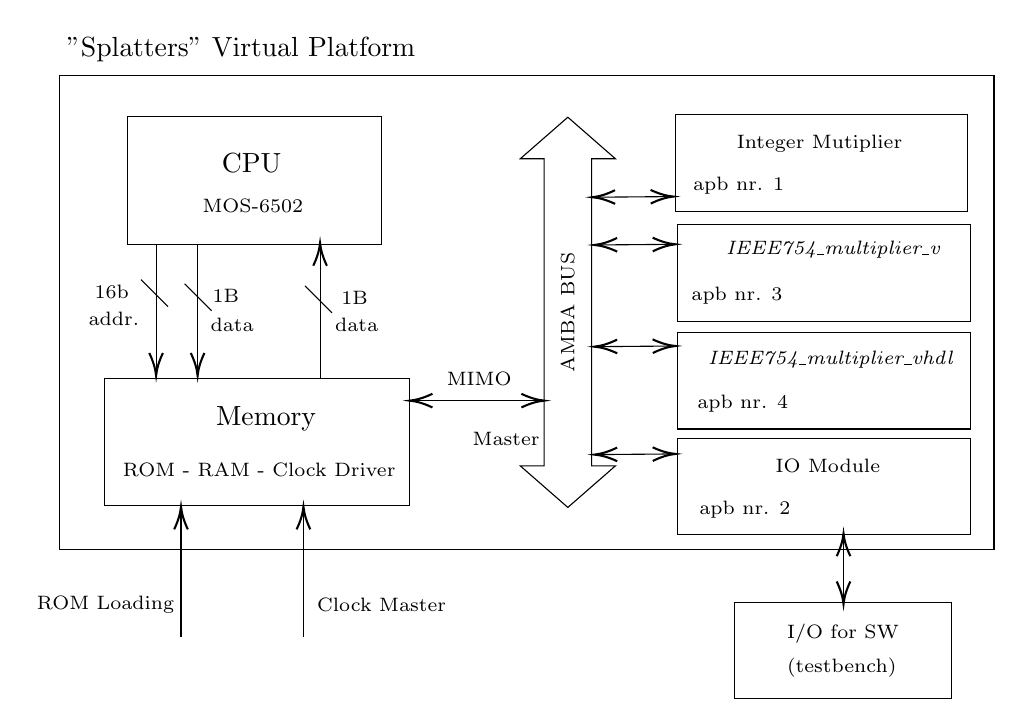
\begin{tikzpicture}[x=0.75pt,y=0.75pt,yscale=-1,xscale=1]
%uncomment if require: \path (0,345.3104705810547); %set diagram left start at 0, and has height of 345.3104705810547

%Shape: Rectangle [id:dp4968396283550932] 
\draw   (53.25,31.54) -- (503.72,31.54) -- (503.72,260) -- (53.25,260) -- cycle ;
%Shape: Rectangle [id:dp3262928051233943] 
\draw   (86.25,51.54) -- (208.5,51.54) -- (208.5,113) -- (86.25,113) -- cycle ;
%Shape: Rectangle [id:dp44477651017849396] 
\draw   (75.25,177.54) -- (222.14,177.54) -- (222.14,239) -- (75.25,239) -- cycle ;
%Straight Lines [id:da795946202356945] 
\draw    (100,113.4) -- (100,174.3) ;
\draw [shift={(100,176.3)}, rotate = 270] [color={rgb, 255:red, 0; green, 0; blue, 0 }  ][line width=0.75]    (10.93,-3.29) .. controls (6.95,-1.4) and (3.31,-0.3) .. (0,0) .. controls (3.31,0.3) and (6.95,1.4) .. (10.93,3.29)   ;

%Straight Lines [id:da836229711939] 
\draw    (120,113.4) -- (120,174.3) ;
\draw [shift={(120,176.3)}, rotate = 270] [color={rgb, 255:red, 0; green, 0; blue, 0 }  ][line width=0.75]    (10.93,-3.29) .. controls (6.95,-1.4) and (3.31,-0.3) .. (0,0) .. controls (3.31,0.3) and (6.95,1.4) .. (10.93,3.29)   ;

%Straight Lines [id:da03787383719669668] 
\draw    (179,114.4) -- (179,177.31) ;

\draw [shift={(179,112.4)}, rotate = 90] [color={rgb, 255:red, 0; green, 0; blue, 0 }  ][line width=0.75]    (10.93,-3.29) .. controls (6.95,-1.4) and (3.31,-0.3) .. (0,0) .. controls (3.31,0.3) and (6.95,1.4) .. (10.93,3.29)   ;
%Straight Lines [id:da34466257749451923] 
\draw    (92.74,130) -- (105.74,143) ;


%Straight Lines [id:da2133300536470074] 
\draw    (113.74,132) -- (126.74,145) ;


%Straight Lines [id:da08023248386644743] 
\draw    (171.74,133) -- (184.74,146) ;


%Straight Lines [id:da7332016414003715] 
\draw    (171,241.4) -- (171,302.3) ;

\draw [shift={(171,239.4)}, rotate = 90] [color={rgb, 255:red, 0; green, 0; blue, 0 }  ][line width=0.75]    (10.93,-3.29) .. controls (6.95,-1.4) and (3.31,-0.3) .. (0,0) .. controls (3.31,0.3) and (6.95,1.4) .. (10.93,3.29)   ;
%Straight Lines [id:da4092830778178417] 
\draw    (112,241.4) -- (112,302.3) ;

\draw [shift={(112,239.4)}, rotate = 90] [color={rgb, 255:red, 0; green, 0; blue, 0 }  ][line width=0.75]    (10.93,-3.29) .. controls (6.95,-1.4) and (3.31,-0.3) .. (0,0) .. controls (3.31,0.3) and (6.95,1.4) .. (10.93,3.29)   ;
%Up Down Arrow [id:dp2817398494023984] 
\draw   (275.48,71.77) -- (298.38,51.77) -- (321.27,71.77) -- (309.82,71.77) -- (309.82,219.77) -- (321.27,219.77) -- (298.38,239.77) -- (275.48,219.77) -- (286.93,219.77) -- (286.93,71.77) -- cycle ;
%Straight Lines [id:da7134872339344482] 
\draw    (284.93,188.32) -- (224.2,188.32) ;
\draw [shift={(222.2,188.32)}, rotate = 360] [color={rgb, 255:red, 0; green, 0; blue, 0 }  ][line width=0.75]    (10.93,-3.29) .. controls (6.95,-1.4) and (3.31,-0.3) .. (0,0) .. controls (3.31,0.3) and (6.95,1.4) .. (10.93,3.29)   ;
\draw [shift={(286.93,188.32)}, rotate = 180] [color={rgb, 255:red, 0; green, 0; blue, 0 }  ][line width=0.75]    (10.93,-3.29) .. controls (6.95,-1.4) and (3.31,-0.3) .. (0,0) .. controls (3.31,0.3) and (6.95,1.4) .. (10.93,3.29)   ;
%Shape: Rectangle [id:dp2727152904351162] 
\draw   (350.25,50.54) -- (491.05,50.54) -- (491.05,97) -- (350.25,97) -- cycle ;
%Shape: Rectangle [id:dp6949852059810868] 
\draw   (351.4,103.54) -- (492.2,103.54) -- (492.2,150) -- (351.4,150) -- cycle ;
%Shape: Rectangle [id:dp8955494647270708] 
\draw   (351.4,155.54) -- (492.2,155.54) -- (492.2,202) -- (351.4,202) -- cycle ;
%Shape: Rectangle [id:dp9609804129587618] 
\draw   (351.4,206.54) -- (492.2,206.54) -- (492.2,253) -- (351.4,253) -- cycle ;
%Straight Lines [id:da3997085908375665] 
\draw    (347.2,90.02) -- (312.2,90.31) ;
\draw [shift={(310.2,90.32)}, rotate = 359.52] [color={rgb, 255:red, 0; green, 0; blue, 0 }  ][line width=0.75]    (10.93,-3.29) .. controls (6.95,-1.4) and (3.31,-0.3) .. (0,0) .. controls (3.31,0.3) and (6.95,1.4) .. (10.93,3.29)   ;
\draw [shift={(349.2,90)}, rotate = 179.52] [color={rgb, 255:red, 0; green, 0; blue, 0 }  ][line width=0.75]    (10.93,-3.29) .. controls (6.95,-1.4) and (3.31,-0.3) .. (0,0) .. controls (3.31,0.3) and (6.95,1.4) .. (10.93,3.29)   ;
%Straight Lines [id:da6466953946936234] 
\draw    (348.2,113.02) -- (313.2,113.31) ;
\draw [shift={(311.2,113.32)}, rotate = 359.52] [color={rgb, 255:red, 0; green, 0; blue, 0 }  ][line width=0.75]    (10.93,-3.29) .. controls (6.95,-1.4) and (3.31,-0.3) .. (0,0) .. controls (3.31,0.3) and (6.95,1.4) .. (10.93,3.29)   ;
\draw [shift={(350.2,113)}, rotate = 179.52] [color={rgb, 255:red, 0; green, 0; blue, 0 }  ][line width=0.75]    (10.93,-3.29) .. controls (6.95,-1.4) and (3.31,-0.3) .. (0,0) .. controls (3.31,0.3) and (6.95,1.4) .. (10.93,3.29)   ;
%Straight Lines [id:da6950140444976091] 
\draw    (348.2,162.02) -- (313.2,162.31) ;
\draw [shift={(311.2,162.32)}, rotate = 359.52] [color={rgb, 255:red, 0; green, 0; blue, 0 }  ][line width=0.75]    (10.93,-3.29) .. controls (6.95,-1.4) and (3.31,-0.3) .. (0,0) .. controls (3.31,0.3) and (6.95,1.4) .. (10.93,3.29)   ;
\draw [shift={(350.2,162)}, rotate = 179.52] [color={rgb, 255:red, 0; green, 0; blue, 0 }  ][line width=0.75]    (10.93,-3.29) .. controls (6.95,-1.4) and (3.31,-0.3) .. (0,0) .. controls (3.31,0.3) and (6.95,1.4) .. (10.93,3.29)   ;
%Straight Lines [id:da40098870426886013] 
\draw    (348.2,214.02) -- (313.2,214.31) ;
\draw [shift={(311.2,214.32)}, rotate = 359.52] [color={rgb, 255:red, 0; green, 0; blue, 0 }  ][line width=0.75]    (10.93,-3.29) .. controls (6.95,-1.4) and (3.31,-0.3) .. (0,0) .. controls (3.31,0.3) and (6.95,1.4) .. (10.93,3.29)   ;
\draw [shift={(350.2,214)}, rotate = 179.52] [color={rgb, 255:red, 0; green, 0; blue, 0 }  ][line width=0.75]    (10.93,-3.29) .. controls (6.95,-1.4) and (3.31,-0.3) .. (0,0) .. controls (3.31,0.3) and (6.95,1.4) .. (10.93,3.29)   ;
%Shape: Rectangle [id:dp9968544630762932] 
\draw   (378.72,285.54) -- (483.2,285.54) -- (483.2,332) -- (378.72,332) -- cycle ;
%Straight Lines [id:da7120898546169434] 
\draw    (431.2,284.37) -- (431.2,254.32) ;
\draw [shift={(431.2,252.32)}, rotate = 450] [color={rgb, 255:red, 0; green, 0; blue, 0 }  ][line width=0.75]    (10.93,-3.29) .. controls (6.95,-1.4) and (3.31,-0.3) .. (0,0) .. controls (3.31,0.3) and (6.95,1.4) .. (10.93,3.29)   ;
\draw [shift={(431.2,286.37)}, rotate = 270] [color={rgb, 255:red, 0; green, 0; blue, 0 }  ][line width=0.75]    (10.93,-3.29) .. controls (6.95,-1.4) and (3.31,-0.3) .. (0,0) .. controls (3.31,0.3) and (6.95,1.4) .. (10.93,3.29)   ;

% Text Node
\draw (141,19) node   [align=left] {"Splatters" Virtual Platform};
% Text Node
\draw (146,74) node   [align=left] {CPU};
% Text Node
\draw (146.65,94.7) node   [align=left] {{\scriptsize MOS-6502}};
% Text Node
\draw (153,197) node   [align=left] {Memory};
% Text Node
\draw (149.65,221.7) node   [align=left] {{\scriptsize ROM - RAM - Clock Driver}};
% Text Node
\draw (195.65,138.7) node   [align=left] {{\scriptsize 1B}};
% Text Node
\draw (133.65,137.7) node   [align=left] {{\scriptsize 1B}};
% Text Node
\draw (78.65,135.7) node   [align=left] {{\scriptsize 16b}};
% Text Node
\draw (196.65,151.7) node   [align=left] {{\scriptsize data}};
% Text Node
\draw (136.65,151.7) node   [align=left] {{\scriptsize data}};
% Text Node
\draw (79.65,148.7) node   [align=left] {{\scriptsize addr.}};
% Text Node
\draw (208.65,286.7) node   [align=left] {{\scriptsize Clock Master}};
% Text Node
\draw (75.65,286.7) node   [align=left] {{\scriptsize ROM Loading}};
% Text Node
\draw (255.65,177.7) node   [align=left] {{\scriptsize MIMO}};
% Text Node
\draw (298.38,145.77) node  [rotate=-270.01] [align=left] {{\scriptsize AMBA BUS}};
% Text Node
\draw (268.65,206.7) node   [align=left] {{\scriptsize Master}};
% Text Node
\draw (419.65,64.7) node   [align=left] {{\scriptsize Integer Mutiplier}};
% Text Node
\draw (380.65,84.7) node   [align=left] {{\scriptsize apb nr. 1}};
% Text Node
\draw (426.65,115.7) node   [align=left] {{\scriptsize \textit{IEEE754\_multiplier\_v}}};
% Text Node
\draw (381.65,137.7) node   [align=left] {{\scriptsize apb nr. 3 }};
% Text Node
\draw (425.27,168.7) node   [align=left] {{\scriptsize \textit{IEEE754\_multiplier\_vhdl}}};
% Text Node
\draw (382.65,189.7) node   [align=left] {{\scriptsize apb nr. 4}};
% Text Node
\draw (423.65,219.7) node   [align=left] {{\scriptsize IO Module}};
% Text Node
\draw (383.65,240.7) node   [align=left] {{\scriptsize apb nr. 2}};
% Text Node
\draw (430.96,308.77) node   [align=left] {{\scriptsize I/O for SW }\\{\scriptsize (testbench)}};


\end{tikzpicture}
			\centering
\caption{Schematic of the Virtual Platform "splatters".}
\label{fig:vpRappresentation}
\end{figure*}



\tikzset{
	->, % makes the edges directed
	>=stealth, % makes the arrow heads bold
	node distance=5cm, % specifies the minimum distance between two nodes. Change if n every state/.style={thick, fill=gray!10}, % sets the properties for each ?state? n initial text=$ $, % sets the text that appears on the start arrow
}

\begin{figure*}[tb]
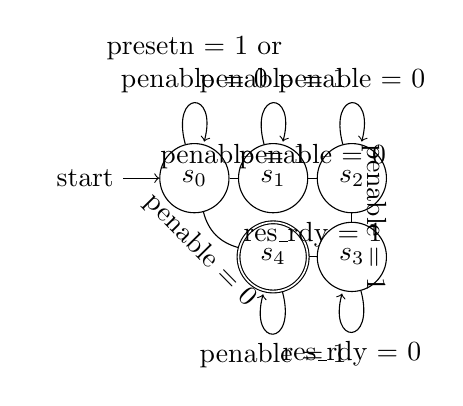
\begin{tikzpicture}

%s0
\node[state, initial] (s0) {$s_0$};		
%s1										
\node[state, right of=s0] (s1) {$s_1$};	
%s2									
\node[state, right of=s1] (s2) {$s_2$};		
%s3								
\node[state, below of=s2] (s3) {$s_3$};
%s4			
\node[state, below of=s1, accepting] (s4) {$s_4$};			


\draw (s0) edge[loop above] node[text width=4cm,align=center]  {presetn = 1 or penable = 0} (s0);

\draw (s0) edge[above] node{penable = 1} (s1);

\draw (s1) edge[above, sloped] node{penable = 0} (s2);
\draw (s1) edge[loop above, sloped] node{penable = 1} (s1);

\draw (s2) edge[above, sloped] node{penable = 1} (s3);
\draw (s2) edge[loop above, sloped] node{penable = 0} (s2);

\draw (s3) edge[above, sloped] node{res\_rdy = 1} (s4);
\draw (s3) edge[loop below, sloped] node{res\_rdy = 0} (s3);

\draw (s4) edge[below, sloped, bend left] node{penable = 0} (s0);
\draw (s4) edge[loop below, sloped] node{penable = 1} (s4);


\end{tikzpicture}
\centering
\caption{Wrapper Toplevel}
\label{fig:wrappertoplevel}
\end{figure*}
\begin{figure*}[tb]
	
	\begin{sequencediagram}
		\newinst [3]{mem}{:Memory} 
		\newinst [3]{per}{:Peripheral} 
		\newinst [3]{mul}{:Multiplier} 
		
		\begin{sdblock}{func}{reset\_flags()}
					\postlevel
					\postlevel
					\begin{messcall}
						{mem}{\shortstack{ pwrite = 0 \\ penable = 0 \\ presetn = 0 \\ pready = 0}}{per}
					\end{messcall}
			\end{sdblock}
		
		
	\begin{sdblock}{op1}{send op1}
			\begin{messcall}
				{mem}{\shortstack{ pwdata = op1}}{per}
			\end{messcall}
		\begin{messcall}
			{mem}{\shortstack{ psel = 4}}{per}
		\end{messcall}
		\begin{messcall}
		{mem}{\shortstack{ penable = 1}}{per}
	\end{messcall}

\end{sdblock}
		\begin{messcall}
	{mem}{\shortstack{ penable = 0}}{per}
\end{messcall}

\begin{sdblock}{op2}{send op2}
			\begin{messcall}
	{mem}{\shortstack{ pwdata = op2}}{per}
\end{messcall}
		\begin{messcall}
	{mem}{\shortstack{ psel = 4}}{per}
\end{messcall}
		\begin{messcall}
	{mem}{\shortstack{ penable = 1}}{per}
\end{messcall}
	\end{sdblock}

		\begin{call}
	{per}{\shortstack{ in\_rdy = 1}}{mul}{res\_rdy = 1}
\end{call}

\begin{sdblock}{res}{send result}
		\postlevel
	\begin{messcall}
		{per}{\shortstack{ prdata = res \\ pready = 1}}{mem}
	\end{messcall}
\end{sdblock}

		\begin{messcall}
	{mem}{\shortstack{ penable = 0}}{per}
\end{messcall}
		\begin{messcall}
	{mem}{\shortstack{ psel = 0}}{per}
\end{messcall}


	\end{sequencediagram}
	\centering
	\caption{Protocol Sequence Diagram}
	\label{fig:seqDiagram}
\end{figure*}





\begin{figure*}[tb]
\centering
\includegraphics[scale=0.60]{figures/UT-10-9-cpu.png}
\caption{CPU screenshoot during $10^9$ simulation with TLM-UT}
\label{fig:ut-cpu}
\end{figure*}
\begin{figure*}[tb]
	\centering
	\includegraphics[scale=0.60]{figures/LT-10-9-cpu.png}
	\caption{CPU screenshoot during $10^9$ simulation with TLM-LT}
	\label{fig:lt-cpu}
\end{figure*}
\begin{figure*}[tb]
	\centering
	\includegraphics[scale=0.60]{figures/AT4-10-9-cpu.png}
	\caption{CPU screenshoot during $10^9$ simulation with TLM-LT}
	\label{fig:at4-cpu}
\end{figure*}
\begin{figure*}[tb]
\centering
\includegraphics[scale=0.60]{figures/RTL-10-9-cpu.png}
\caption{CPU screenshoot during $10^9$ simulation with TLM-RTL}
\label{fig:rtl-cpu}
\end{figure*}

\begin{figure*}[tb]
	\centering
	\includegraphics[scale=0.33]{figures/verilog.png}
	\caption{Waves of verilog}
	\label{fig:verilog}
\end{figure*}

\begin{figure*}[tb]
	\centering
	\includegraphics[scale=0.33]{figures/verilog-zoom.png}
	\caption{Waves of verilog zoom}
	\label{fig:verilogzoom}
\end{figure*}


\begin{figure*}[tb]
	\centering
	\includegraphics[scale=0.33]{figures/verilog-binding.png}
	\caption{Waves of verilog zoom}
	\label{fig:verilogbinding}
\end{figure*}


\begin{figure*}[tb]
	\centering
	\includegraphics[scale=0.50]{figures/longwave.png}
	\caption{Waves of verilog zoom}
	\label{fig:longsimulation}
\end{figure*}

	
	
\end{document}